
\refstepcounter{Exercise}
\clearpage\subsection*{\theExercise CGIでセンサーの情報を表示させる}
\addtocounter{Exercise}{-1}\refstepcounter{Exercise}\label{E:Sensors}

% \clearpage\subsection*{CGIでセンサーの情報を表示させる}
考え方

温度、温度、\ruby{気圧}{きあつ}、照度センサーの情報をCGIを使ってウェブページから見れるようにしましょう。


\bigskip

まずは、プログラム実行してみましょう。

ブラウザを開いて、

localhost:3000/cgi-bin/sensors.hsp

にアクセスしてください。


%
%スクショ
%ブラウザで開いたときの
%koyaman
%September 20, 2019 2:37 AM


\centering
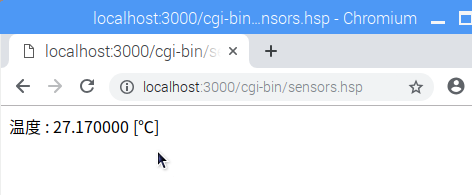
\includegraphics[width=0.75\textwidth]{text07-img/ome7-img058.png}
\flushleft


温度センサーの値が表示されていると思います。

リロードするたびに値が更新されます。

今は温度センサーしか表示をしていないので、他のセンサーの値も表示させるように変更してみましょう。

%
%その他のセンサーを表示させた完成図のスクショ
%koyaman
%September 20, 2019 2:45 AM


\centering
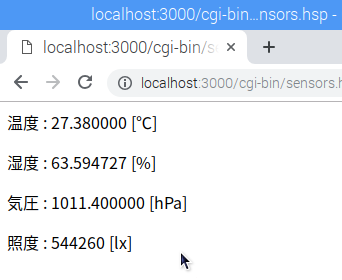
\includegraphics[width=0.75\textwidth]{text07-img/ome7-img059.png}
\flushleft

次にプログラムを見てみましょう。


\clearpage
プログラム解説





\begin{table}[htbp]
    \centering
    % \caption{文字タイプ表}
    \begin{tabular}{|l|}
        \hline
        
        1. \#include {\textquotedbl}rpz-gpio-cl.as{\textquotedbl}\\ 
        2. \#include {\textquotedbl}hsp3cl.as{\textquotedbl}\\
        3. 
        4. mes {\textquotedbl}Content-type: text/html{\textbackslash}n{\textquotedbl}\\
        5. mes {\textquotedbl}{\textless}html{\textgreater}{\textless}head{\textgreater}{\textless}meta charset={\textbackslash}{\textquotedbl}utf-8{\textbackslash}{\textquotedbl}{\textgreater}{\textless}/head{\textgreater}{\textless}body{\textgreater}{\textquotedbl}\\
        6. \\
        7. i2c\_ch\_bme\ = \ 0 \\
        8. i2c\_ch\_tsl \ = \ 1 \\
        9. \\
        10. fail \ = \ init\_bme(i2c\_ch\_bme)\ \ \ \ ; 温\ruby{湿}{しつ}度気圧センサ bm280を初期化する \\
        11. if fail \{\ \ \ \ \ \ \ \ \ \ \ \   ; 初期化成功チェック \\
        12. \ \ mes {\textquotedbl}failed to init bme: {\textquotedbl} + fail \\
        13. \ \ end \\
        14. \} \\
        15. \\
        16. init\_lux i2c\_ch\_tsl\ \ \ \ \ \ ; 照度センサ tsl2572を初期化する\\
        17. \\
        18. *main \\
        19. \ \ temp = get\_temp(i2c\_ch\_bme)\ \ \ \ ; 温度取得\\
        20. \ \ hum \ = get\_hum(i2c\_ch\_bme)\ \ \ \ ; 湿度取得\\
        21. \ \ press= get\_press(i2c\_ch\_bme)\ \ \ \ ; 気圧取得\\
        22. \ \ lux \ = get\_lux(i2c\_ch\_bme)\ \ \ \ ; 照度取得\\
        23. \\
        24. \\
        25. \ \ ; 取得したデータの表示\\
        26. \ \ mes {\textquotedbl}{\textless}p{\textgreater}温度 : {\textquotedbl} + temp + {\textquotedbl} [℃]{\textless}/p{\textgreater}{\textquotedbl}\\
        27. \\
        28. \ \ \ \ mes {\textquotedbl}{\textless}/body{\textgreater}{\textless}/html{\textgreater}{\textquotedbl}\\
        29. end\\
        \hline
    \end{tabular}
\end{table}

\flushleft
この例題は{\textasciitilde}/03/sensors.hspをもとにしています。詳しい解説はそちらを参照してください。

19~22行目で温度、湿度、気圧、照度センサーから情報を取得しています。

結果はそれぞれtemp, hum, press,
lux変数へ入っています。

26行目で、温度センサーの値をpタグで表示しています。

\bigskip


\bigskip


\bigskip

\clearpage
\refstepcounter{Question}\theQuestion\label{Q:sensors}

% 問題7-14  
% 友達のCGIへアクセスして、センサーの値を確認してみよう。

温度センサーと同様に、湿度、気圧、照度センサーの値も表示させてみましょう。



\begin{table}[htbp]
    \centering
    % \caption{文字タイプ表}
    \begin{tabular}{|c|}
        \hline
        localhost:3000/cgi-bin/sensors\_table.hsp\\
        \hline
    \end{tabular}
\end{table}

にブラウザでアクセスをしてみましょう。

温度センサーの値が表形式で表示されたと思います。

%
%スクショ
%実行画面
%localhost:3000/cgi{}-bin/sensors\_table.hsp
%koyaman
%September 20, 2019 2:44 AM


\centering
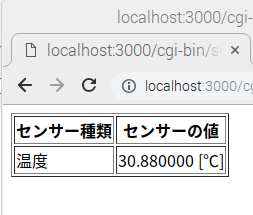
\includegraphics[width=0.8\textwidth]{text07-img/ome7-img060.png}
\flushleft

次は、湿度、気圧、照度センサーの値を表形式で表示するように変更してみましょう。
